\section{Axiomatic Design}

The axiomatic design framework was developed in the late \(20^{th}\) century by Professor Nam P. Suh while at MIT
and the NSF \cite{suh}.  This was in response to concern in the engineering community that \emph{design} was being
practiced almost exclusively as an ad-hoc creative endeavor with very little in the way of scientific discipline.
In the words of Professor Suh:
\begin{quote}
  It [design] might have preceding the development of natural sciences by scores of centuries.  Yet, to this day,
  design is being done intuitively as an art.  It is one of the few technical areas where experience is more
  important than formal education.
\end{quote}
It is important to note that Professor Suh was not making these claims in an educational vacuum, but in the shadow
of several recent major design failures such as the Union Carbide plant disaster in India, nuclear power plant
accidents at Three Mile Island and Chenobyl, and the Challenger space shuttle O-ring failure.  Furthermore,
Professor Suh asserts that design-related issues resulting in production problems and operating failures were
increasingly happening in everything from consumer products to big-ticket items.

The following sections provide an overview of axiomatic design as specified in detail by Professor Suh in \cite{suh},
and summarized in \cite{cavallaro,jahanbekam,suh2}.  Following is a description of how the proposed algorithm can be
a helpful tool to a designer using the axiomatic design framework.

\subsection{Design}

\emph{Design} is defined as the process by which it is determined \emph{what} needs to be achieved and then
\emph{how} to achieve it.  Thus, the decisions on what do to are just as important as how to do it.  Creativity is
the process by which experience and intuition are used to generate solutions to perceived needs.  This includes
pattern matching to and adapting existing solutions and synthesizing new solutions.  Thus, creativity plays a vital
role in design.  Since different designers may approach the same problem differently, their level of creativity may
lead to very different, yet plausible, solutions.  Thus, there needs to be a design-agnostic method for comparing
different designs with the goal of selecting the best one.

This discussion will sound very familiar to mathematicians, since creativity is very important for solving math
problems, and in particular, for writing proofs.  Starting with the work of Peano in the \(19^{th}\) century, the
field of mathematics has established various tests on what constitutes a good proof.  For example:
\begin{itemize}
\item Does every conclusion result by proper implication from existing definitions, axioms, and previously-proved
  conclusions?
\item Is direct proof, contrapositive proof, proof by contradiction, or proof by induction the best approach for a
  particular problem?
\item Do proofs by induction contain clear basic, assumptive, and inductive steps?
\item Are all subset and equality relationships properly proved via membership implication?
\item Are all necessary cases included and stated in a mutually exclusive manner?
\item Are degenerate cases sufficiently highlighted?
\item Are all equivalences proved in a proper circular fashion?
\item Are key and reused conclusions highlighted in lemmas?
\end{itemize}
In short, Professor Suh was looking for a similar framework for the more general concept of design.

\subsection{The Framework}

The \emph{best} design among a set of choices is the design that:
\begin{enumerate}
\item exactly satisfies a clearly defined set of needs.
\item has the greatest probability of success.
\end{enumerate}

In a desire to not hinder the creative element needed for design, yet provide some methodology to distinguish bad
designs from good designs from better designs, the diagram in Figure \ref{fig:design} establishes the overall
framework for axiomatic design.

\begin{figure}[h]
  \label{fig:design}
  \begin{center}
    \scalebox{0.75}{
      \begin{tikzpicture}[>=latex',every text node part/.style={align=center}]
        \node (cn) [draw,terminal] at (0,0) {customer \\ needs};
        \node (pd) [draw,process,right=of cn] {problem \\ definition};
        \node (cp) [draw,process,right=2cm of pd] {creative \\ process};
        \node (ap) [draw,process,right=2cm of cp] {analytical \\ process};
        \node (uc) [draw,process,right=of ap] {ultimate \\ check};
        \node (fd) [draw,terminal,right=of uc] {final \\ design};
        \draw [->] (cn) -- (pd);
        \draw [->] (pd) -- node [auto] {FRs} (cp);
        \draw [->] (cp) -- node [auto] {candidate \\ design} (ap);
        \draw [->] (ap) -- (uc);
        \draw [->] (uc) -- (fd);
        \draw [->] (ap) -- ($(ap) + (0,-1.5cm)$) -| (cp);
      \end{tikzpicture}
    }
  \end{center}
  \caption{Axiomatic Design Framework}
\end{figure}

Design starts with the desire to fulfill a clear set of \emph{customer needs}.  The term \emph{customer} refers to
any entity that expresses needs, and can be as varied as individuals, organizations, or society.  The designer, in
the \emph{problem definition} phase, determines how these customer needs will be meet by generating a list of
\emph{functional requirements} (FRs).  It is this list of FRs that determines exactly \emph{what} is to be
accomplished.

Once the set of FRs has been determined, the designer begins the \emph{creative process} by mapping the FRs into
solutions that are embodied in so-called \emph{design parameters} (DPs).  The design parameters contain all of the
information on \emph{how} the various FRs are fulfilled: parts lists, drawings, specifications, etc.  The FRs exist
in a design-agnostic \emph{functional space} and the DPs exist in a solution-specific \emph{physical space}.  It is
the designer's job to provide the most efficient mapping between the two spaces.  This process is represented by
Figure \ref{fig:mapping}.

\begin{figure}[h]
  \label{fig:mapping}
  \begin{center}
    \begin{tikzpicture}[>=latex',every text node part/.style={align=center}]
      \node (fs) [draw,cloud] at (0,0) {FR1 \\ FR2 \\ FR3 \\ \vdots};
      \node [below=1ex of fs] {functional \\ space};
      \node (ps) [draw,cloud,right=1.5in of fs] {DP1 \\ DP2 \\ DP3 \\ \vdots};
      \node [below=1ex of ps] {physical \\ space};
      \draw [->] (fs) to [bend left=45] (ps);
      \draw [->] (fs) to [bend left=30] (ps);
      \draw [->] (fs) to [bend right=30] (ps);
      \draw [->] (fs) to [bend right=45] (ps);
      \draw [->] (fs) -- node [auto] {mapping} (ps);
    \end{tikzpicture}
  \end{center}
  \caption{Mapping FRs to DPs}
\end{figure}

Simple problems may require only one level of FRs; however, more complicated designs may require a hierarchial
structure of FRs, from more general to more detailed requirements.  This type of design if oftern referred to as
\emph{top-down} design.  Each individual FR layer has its own DP mapping.  In fact, the mapping process on one
level should be completed prior to determining the FRs for the next level.  This is because DP choices on one level
may affect choices on the next level.  For example, consider an FR related to a moving part in a design.  The DP
for this FR could specify that the part be moved manually or automatically.  Each choice would result in different
FRs for the actual mechanism selected by the DP.

The FR/DP mapping at each level in the design hierarchy is described by the \emph{design equation}, which is shown
in Equation \ref{eqn:design}.
\begin{equation}
  \label{eqn:design}
  [\FR]=[\text{A}][\DP]
\end{equation}
The design equation is a matrix equation that maps a vector of \(m\) FRs to a vector of \(n\) DPs via an \(m\times
n\) design matrix A.  As will be shown, good designs require \(m=n\), and thus the design matrix is a square
\(n\times n\) matrix.  A full discussion of the design matrix element values is beyond the scope of this research.
Instead, we will use the following two values:
\[A_{ij}=\begin{cases}
X, & \FR_i\ \text{depends on}\ \DP_j \\
0, & \FR_i\ \text{does not depend on}\ \DP_j
\end{cases}\]

Since the FR/DP mapping is non-unique, there needs to be a method to compare different plausible designs so that
the best design can be selected as the final design.  Thus, the framework in Figure \ref{fig:design} includes an
\emph{analytical process} where designs are judged by a set of axioms, corollaries, and theorems that specify the
properties common to all good designs.  Once the best design, according to this analysis, is selected, it undergoes
an \emph{ultimate check} to make sure that it sufficiently meets all of the customer's needs.  If so, then that
design is selected as the final design.

\subsection{The Axioms}

The analytical process is based on two major axioms: the independence axiom and the information axiom.  This section
describes these axioms and their related corollaries and theorems.

The independence axiom imposes a restriction on the FR/DP mapping:

\begin{axiom}[Independence]
  \label{axm:independ}
  An optimal design always maintains the independence of the FRs.  This means that the FRs and DPs are related in
  such a way that a specific DP can be adjusted to satisfy its corresponding FR without affecting other FRs.
\end{axiom}

The ideal case is when the design matrix is a diagonal matrix, and so each FR is mapped to and is satisfied by
exactly one DP.  This is referred to as an \emph{uncoupled} design, which is demonstrated in Figure
\ref{fig:uncoupled}.  Uncoupled designs completely adhere to the independence axiom.

\begin{figure}[h]
  \label{fig:uncoupled}
  \begin{equation*}
    \begin{bmatrix}
      \FR1 \\ \FR2 \\ \FR3
    \end{bmatrix}=\begin{bmatrix}
    X & 0 & 0 \\
    0 & X & 0 \\
    0 & 0 & X \\
    \end{bmatrix}\begin{bmatrix}
      \DP1 \\ \DP2 \\ \DP3
    \end{bmatrix}
  \end{equation*}
  \caption{An Uncoupled Design}
\end{figure}

The next best situation is when the design matrix is a lower-triangular matrix.  The idea is to finalize the first
DPs before moving on to the later DPs.  Thus, \(\text{DP}_i\) can be adjusted without affected \(\FR_1\) through
\(\FR_{i-1}\).  This is referred to as a \emph{decoupled} design, which is demonstrated in Figure
\ref{fig:decoupled}.  Although decoupled designs do not completely adhere to the independence axiom, they may be
reasonable compromises in designs that address complex problems.

\begin{figure}[h]
  \label{fig:decoupled}
  \begin{equation*}
    \begin{bmatrix}
      \FR1 \\ \FR2 \\ \FR3
    \end{bmatrix}=\begin{bmatrix}
    X & 0 & 0 \\
    X & X & 0 \\
    X & X & X \\
    \end{bmatrix}\begin{bmatrix}
      \DP1 \\ \DP2 \\ \DP3
    \end{bmatrix}
  \end{equation*}
  \caption{A Decoupled Design}
\end{figure}

The worst solution is a non-triangular matrix where every change in a DP affects multiple FRs both before it and
after it.  This is referred to as a \emph{coupled} design, which is demonstrated in Figure \ref{fig:coupled}.
Coupled designs are in complete violation of the independence axiom and generally should be decoupled by reworking
the FRs or adding additional DPs.  Unfortunately, adding additional DPs runs counter to the second axiom.

\begin{figure}[h]
  \label{fig:coupled}
  \begin{equation*}
    \begin{bmatrix}
      \FR1 \\ \FR2 \\ \FR3
    \end{bmatrix}=\begin{bmatrix}
    X & X & X \\
    X & X & X \\
    X & X & X \\
    \end{bmatrix}\begin{bmatrix}
      \DP1 \\ \DP2 \\ \DP3
    \end{bmatrix}
  \end{equation*}
  \caption{A Coupled Design}
\end{figure}

\begin{axiom}[Information]
  The best design is a functionally uncoupled design that has the minimum information content.
\end{axiom}

The \emph{Information} contained in a particular DP is inversely related to the probability that the DP can
successfully fulfill its corresponding FR(s) by Equation \ref{eqn:info}.
\begin{equation}
  \label{eqn:info}
  I=\log_2\left(\frac{1}{p}\right)
\end{equation}
where \(p\) is the probability of success and \(I\) is measured in bits.  This probability must take into
consideration such things as tolerances, ease of manufacture, failure rates, etc.  The information content of a
design is then the sum of the information content of the individual DPs.

From these two axioms come the following seven corollaries:
\begin{description}
\item[Corollary 1:] Decouple or separate parts or aspects of a solution if the FRs are coupled or become
  interdependent in the designs proposed.
\item[Corollary 2:] Minimize the number of FRs.
\item[Corollary 3:] \label{cor:integrate} Integrate design features in a single physical part if FRs can be
  independently satisfied in the proposed solution.
\item[Corollary 4:] Use standardized or interchangeable parts if the use of these parts is consistent with the FRs.
\item[Corollary 5:] Use symmetrical shapes and/or arrangements if they are consistent with the FRs.
\item[Corollary 6:] Specify the largest allowable tolerance in stating FRs.
\item[Corollary 7:] Seek an uncoupled design that requires less information that coupled designs in satisfying a
  set of FRs.
\end{description}

We will now consider the theorems that arise from these axioms and corollaries that prove the optimal design results
from a square design matrix.  In other words, the number of FRs \(m\) should be equal to the number of DPs \(n\).
First, consider the case where \(m>n\).  Intuitively, this forces a single DP to be mapped to multiple FRs.
Otherwise, some FRs cannot be satisfied by the DPs.  This result is stated in Theorem \ref{thm:frgtdp}.

\begin{theorem}
  \label{thm:frgdp}
  When the number of DPs is less that the number of FRs, either a coupled design results of the FRs cannot be
  satisfied.
\end{theorem}

The solution to this problem is given by Theorem \ref{thm:adddp}.
\begin{theorem}
  \label{thm:adddp}
  A coupled design due to more FRs than DPs can be decoupled by adding new DPs if the additional DPs result in a
  lower triangular design matrix.
\end{theorem}

An example is show in Figure \ref{fig:dcexample}.  Note that the addition of DP3 results in a decoupled design.

\begin{figure}[h]
  \label{fig:dcexample}
  \[\begin{bmatrix}
  \FR1 \\ \FR2 \\ \FR3
  \end{bmatrix}=\begin{bmatrix}
  X & 0 \\
  X & X \\
  X & X \\
  \end{bmatrix}\begin{bmatrix}
    \DP1 \\ \DP2 \\
  \end{bmatrix}\implies\begin{bmatrix}
  \FR1 \\ \FR2 \\ \FR3
  \end{bmatrix}=\begin{bmatrix}
  X & 0 & 0 \\
  X & X & 0 \\
  X & X & X \\
  \end{bmatrix}\begin{bmatrix}
    \DP1 \\ \DP2 \\ \DP3
  \end{bmatrix}\]
  \caption{Decoupling by Adding DPs}
\end{figure}

The case where the number of FRs is less than the number of DPs is covered by Theorem \ref{thm:frltdp}.

\begin{theorem}
  \label{thm:frltdp}
  When there are less FRs than DPs then the design is either coupled or redundant.
\end{theorem}

Finally, the previous three theorems result in the conclusion in Theorem \ref{freqdp}.

\begin{theorem}
  \label{thm:freqdp}
  In an ideal design, the number of FRs is equal to the number of DPs.
\end{theorem}

\subsection{Part Consolidation}

One particular area of design focus is the number of parts in a product design.  According to Professor Suh:
\begin{quote}
  Poorly designed products often cost more because they use more materials or parts than do well-designed products.
  They are often difficult to manufacture and maintain.
\end{quote}
Decreasing the number of parts in a design while maintaining the independence of the FRs, consistent with Corollary
\ref{cor:integrate}, lowers the information content of the design.  An informative example is the combination
can/bottle opener shown in Figure \ref{fig:opener}.

\begin{figure}[h]
  \label{fig:opener}
  \begin{center}
    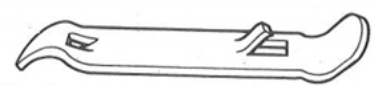
\includegraphics{opener}
  \end{center}
  \caption{Part Consolidation Example}
\end{figure}

The design of this handy utensil has two FRs:

\begin{description}
\item[FR1:] Open beverage cans
\item[FR2:] Open beverage bottles
\end{description}

Both FRs are consolidated into a single part, yet remain independent as long as there is no desire to open a can and
a bottle simultaneously.

The goal of this research is to provide designers with a tool that they can use to determine the minimum number of
parts required to realize a particular design at a particular level of the FR hierarchy.  The designer is required
to construct a graph where the vertices are the FRs and the edges indicate that the endpoint FRs need to be
realized by separate parts due to independence or other reason.  Note that how the edges are determined is beyond
the scope of this research.  Adjacent FRs are candidates for part consolidation.  The goal is to find the chromatic
number of the resulting graph, which corresponds to the minimum number of parts.

Unfortunately, finding the chromatic number of a graph is known to be an NP-hard problem.  Thus, an algorithm is
proposed with improved runtime complexity that can be run on a computer in order to provide a designer with an
answer in a reasonable amount of time.  Designs with different minimum part requirements can then be compared
during the analytical process as part of the overall process of selecting the best design.
